\documentclass[conference]{IEEEtran}
\IEEEoverridecommandlockouts
% The preceding line is only needed to identify funding in the first footnote. If that is unneeded, please comment it out.
\usepackage{cite}
\usepackage{amsmath,amssymb,amsfonts}
\usepackage{algorithmic}
\usepackage{graphicx}
\usepackage{textcomp}
\usepackage{xcolor}
\def\BibTeX{{\rm B\kern-.05em{\sc i\kern-.025em b}\kern-.08em
    T\kern-.1667em\lower.7ex\hbox{E}\kern-.125emX}}
\begin{document}
\title{Sporadic server scheduling in Real-Time operating systems\\
}

\author{\IEEEauthorblockN{ Andrew Zakhary}
\IEEEauthorblockA{\textit{Electronics Engineering} \\
\textit{Hochschule Hamm-Lippstadt}\\
Hamm, Germany \\
2210009}
}

\maketitle

\begin{abstract}

\end{abstract}

\begin{IEEEkeywords}
component, formatting, style, styling, insert
\end{IEEEkeywords}

\section{Introduction}
The term "Real time operating systems (RTOS)" describes operating systems where the execute of the tasks have to take into consideration the time constraints. These types of operating systems are used in time-critical applications as energy generation facilities, medical devices, motor drivers, etc. Real time systems have some features that set them apart from other operating systems. These features include:
\begin{itemize}
    \item \textbf{Determinism}: RTOS is deterministic by nature. This means that tasks must and will be executed within a pre-specified deadline. Unlike other operating systems where tasks are only processed sequentially.
    \item \textbf{Schedulability}: RTOS are designed to use algorithms that decide in what order can the processes run while maintaining that every task is done before their deadline. The ability of doing this is called being "schedulable". These algorithms could be split further into two groups:
    \begin{itemize}
        \item \textbf{Preemptive}: These are scheduling algorithms that can interrupt the running task to run another task instead that it deemed with a higher priority. Examples of these algorithms are Round-Robin, Priority Scheduling and Longest remaining Job First.
        \item \textbf{Non-preemptive}: these and algorithms that run each task to their end without interrupting and only then can proceed with the next task. Examples of these are Shortest Job First, Longest Job First and First Come First Served.
    \end{itemize}
\end{itemize}
These RTOSs can also be split into different categories depending on the application where it's used into different categories as follows: 
\begin{itemize}
    \item \textbf{Hard}: Hard RTOS are systems where failure in meeting the deadline in one of the results could lead to catastrophic failures in the systems that may be even deadly. This could be seen in systems as aircraft landing systems.
    \item \textbf{Firm}: Firm RTOS are systems where the failure in meeting one of the deadlines doesn't cause any harm by itself but the result would be useless to the system. Example of this could be found in industrial automation where occasional misses of the system could be tolerated but if they occurred frequently enough the whole system could fail.
    \item \textbf{Soft}: Soft RTOS are systems where the failure in meeting one of the deadlines doesn't lead to any harm but is undesirable. This could be related to performance or quality of service in applications like streaming services where a delay in the system could result in a worse experience for the user but the system would remain functional.
\end{itemize}
As a result of these varying application constrains a lot of different methods of scheduling tasks inside the OS have been developed. In this paper we will review one of them, namely Sporadic Server (SS) scheduling which is built on the Fixed-Priority Server concept.
\section{Background}
\subsection{Fixed-Priority Server}
tasks in an RTOS could be seen as two categories as follows:
\begin{itemize}
    \item \textbf{Periodic tasks}:These are tasks that occur regularly according to predictable intervals. Sensor data acquisition is an example of this as readings from the sensor come at a regular interval.
    \item \textbf{Aperiodic tasks}: These are tasks that unpredictable and can occur at any time during execution. Event-driven changes as user inputs or button presses are an example of this as they can happen at any time and cannot be predicted.
    \item \textbf{Sporadic tasks}: These are a special type of Aperiodic tasks that occur irregularly but still have a pre-known minimum time interval between their arrival time. These could be seen in interrupt handlers that occur irregularly but not more frequently than a pre-known rate.
\end{itemize}
Since RTOSs require to guarantee the schedulability of tasks assuming worst-case conditions \cite{rtosbehaviour}, trying to handle aperiodic and periodic tasks makes guaranteeing this before running the system (i.e. offline guarantee) impossible. On the other hand handling periodic and sporadic tasks could be guaranteed assuming knowing the minimum arrival time of these sporadic tasks. This would allow the realization of all types (i.e. Hard, Soft and Firm) RTOS types.

Handling period and aperiodic tasks could be guaranteed during the running of the OS (i.e. online guarantee) by checking each aperiodic task first as an individual and seeing if it could be scheduled. As a result of this check the algorithm either queues the task to be executed or skips it. As a result this allows only the realization of Firm RTOS.

Fixed-Priority Server scheduling algorithms try to schedule the set of periodic tasks according to a fixed-priority system as Rate-Monotonic (RM) algorithm (in case of SS).
\subsection{Rate Monotonic}
Rate Monotonic is a preemptive scheduling algorithm used to schedule periodic tasks. RM organizes tasks so that the priority is inversely proportional to the period of this task. As the periods are fixed it follows that the priorities are also fixed. This makes the RM a fixed priority scheduling algorithm.

As an example, assume a set of tasks as shown in the Table \ref{tab:RMtaskstable} to be scheduled using RM.
\begin{table}[h]
    \centering
    \begin{tabular}{ |c|c|c| } 
    \hline
        Process ($P$) & Execution Time ($C$) & Period ($T$)\\
        \hline\hline
         ${P_1}$& 3 & 20 \\
         \hline
         ${P_2}$& 2 & 5 \\
         \hline
         ${P_3}$& 2 & 10 \\
         \hline
         
    \end{tabular}
    \vspace{1em}
    \caption{Tasks to be scheduled with RM}
    \label{tab:RMtaskstable}
\end{table}
First a schedulability check needs to be made for the tasks to be executed.This is done using the formula \ref{utilization} as proven by Liu and Layland \cite{schedulingformula} where $n$ is the number of processes to be scheduled and C and T are the execution and period time respectively.
\begin{equation}
    {U}={{\sum^{n}_{i=1}}} \frac{C_i}{T_i} \leq n(2^{1/n}-1)
    \label{utilization}
\end{equation}
Using this equation it is seen that Equation \ref{aRm} is indeed less than Equation \ref{bRM}. This means that these 3 tasks are schedulable under RM.
\begin{equation}
    U=\frac{3}{20}+\frac{2}{5}+\frac{2}{10}=0.75
    \label{aRm}
\end{equation}
\begin{equation}
    n(2^{1/n}-1)=3( 2^{1/3} - 1) = 0.7977
    \label{bRM}
\end{equation}
The LCM of the periods (20,5,10) is calculated which is 20 which would be the scheduling time. Then the priority is set, as mentioned before it's inversely proportional to the period so this means the priorities are set as \(P_2 > P_3 > P_1\)
\begin{figure}[h]
    \centering
    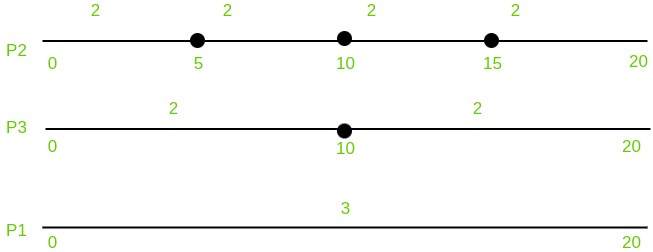
\includegraphics[scale=0.3]{RM overview.png}
    \caption{Tasks with their period and execution time denoted}
    \label{fig:RMoverview}
\end{figure}
The Fig. \ref{fig:RMoverview} shows how the period and the execution time relate. As an example $P_3$ will be executed every 10 units of time and each time with execution time of 2 units.

The algorithm starts then by running the task with the task with the highest priority (i.e. $P_2$) and executes it for 2 units of time uninterrupted. Then $P_3$ is executed for another 2 units of time uninterrupted. After that it's $P_1$'s turn to run but it can only run for 1 unit until it gets preempted and $P_2$ is executed again for another 2 units as it's period has restarted. Since $P_3$'s period has not restarted yet and it was completely executed the algorithm re-executes $P_1$ as it has 2 units of time remaining. Now, all tasks are completely run so nothing is going to be executed until $T=10$. Then the period of $P_2$ and $P_3$ restarts so $P_2$ will run first until $T=12$ and then $P_3$ will run until $T=14$. After that, again all tasks are executed in full so the algorithm doesn't run anything until $T=15$ after which the period of $P_2$ is restarted and it runs until $T=17$ and then stays without running anything until $T=20$. At this point the whole period of 20 units is passed and the pattern repeats. This process could visualised in Fig. \ref{fig:rmTimetable}
\begin{figure}
    \centering
    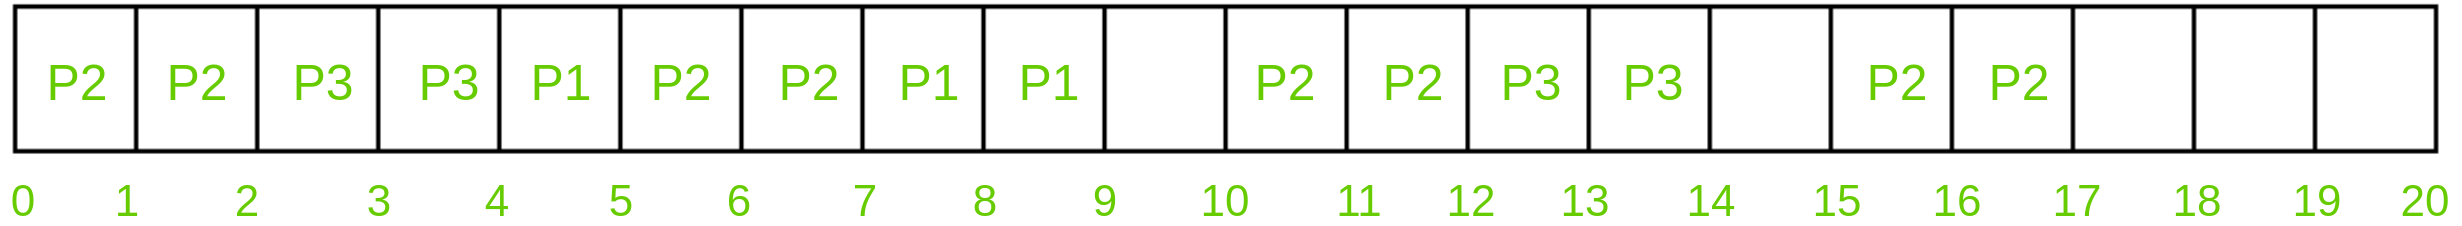
\includegraphics[scale=0.1]{rmtimetable.png}
    \caption{Period of execution using RM algorithm}
    \label{fig:rmTimetable}
\end{figure}
\subsection{Server mechanism}
The sporadic server was introduced by Sprunt, Sha and Lehoczky from Carnegie Mellon University in 1989. The SS algorithm tries to handle aperiodic tasks by creating a high priority task that serves the  incoming aperiodic task. This server would have a capacity ${C_s}$ that is used up whenever an aperiodic task is executed. This capacity is only replenished after a it has been consumed by a period of time $T_s$. The working of SS algorithm contains also some terminologies\cite{SpruntoSS} that could be explained as follows:
\begin{itemize}
    \item \textbf{$P_s$} This represents the priority of the task currently being executed by the system.
    \item \textbf{$P_i$} This represents the priority of a specific task. Priorities are organized in an ascending order. So $P_1$ has higher priority than $P_2$.
    \item \textbf{Active} A description of a priority of a specific task. The task with priority $P_i$ is said to be "active" if $P_s$ is equal to or higher than $P_i$.
    \item \textbf{Idle} A description of a priority of a specific task, similar to "active" but an opposite. The task with priority $P_i$ is said to be "active" if $P_s$ is lower than $P_i$.
    \item \textbf{RT} Represents the replenishment time for the server. This is where the capacity of the server is restocked.
    \item \textbf{RA} Represents the replenishment amount. this is the amount the capacity is replenished by after $RT$ time.
\end{itemize}
The replenishment time $RT$ is set whenever the SS is \textit{active} and is has capacity ($C_s>0$). let the time where the SS started being \textit{active} is $T_A$ then $RT = T_A + T_s$.
The replenishment amount $RA$ is set whenever the SS is switching from \textit{active} to \textit{idle}. let the time when the SS switches from \textit{active} to \textit{idle} is $T_I$ then $RA$ is the capacity consumed in the time frame [$T_A,T_I$].
\subsection{High priority SS example}
Given the set of tasks shown in Table \ref{tab:high priority ss table} it is noticeable that according the RM rules mentioned earlier the priorities could be organized as follows $P_{ss}> \tau_1>\tau_2$. The schedulability could also be tested according to Equation \ref{utilization} to be $U=\frac{1}{6}+\frac{2}{10}+\frac{6}{14}=0.7952 < 0.7797$ 

Since, however the SS is only executed when there's an aperiodic task, the scheduler must start by executing $\tau_1$. This is executed for only one unit of time and then preempted when the aperiodic request \#1 is received as shown in Fig. \ref{fig:high priority ss graph}. At this time (T=1) the SS switches from \textit{idle} to \textit{active} ($T_A = 1$) and executes the request for another one time unit. The capacity is dropped by 1 during this period so $RA$ is set to 1 and since $RT = T_A + T_s$ it follows that $RT= 1+5=6$. After this $\tau_1$ continues the remaining 1 unit of time and then the scheduler executes $\tau_2$ for 5 units of time until this is also preempted by aperiodic request \#2. Again, the SS is \textit{active} at T=8 and executes for 1 unit of time. As mentioned before $RT= 8+1=9$ and $RA=1$. After that $\tau_2$ continues executing for the remaining 1 unit of time of it's execution time. $\tau_1$ is not active again is its period is repeating (T=10) so it executes again for 2 units of time. After that the scheduler is free for 2 units of time as both $\tau_1$ and $\tau_2$ are both executed to completion in this period and there are no aperiodic requests. The scheduler would then continue executing $\tau_2$ when its period repeats at T=14 until T=20 where it would execute the higher priority $\tau_1$.
\begin{table}[h]
    \centering
    \begin{tabular}{ |c|c|c| } 
    \hline
        Process ($P$) & Execution Time ($C$) & Period ($T$)\\
        \hline\hline
         ${SS}$& 1 & 5 \\
         \hline
         ${\tau_1}$& 2 & 10 \\
         \hline
         ${\tau_2}$& 6 & 14 \\
         \hline
         
    \end{tabular}
    \vspace{1em}
    \caption{High-priority example of SS}
    \label{tab:high priority ss table}
\end{table}
\begin{figure}[h]
    \centering
    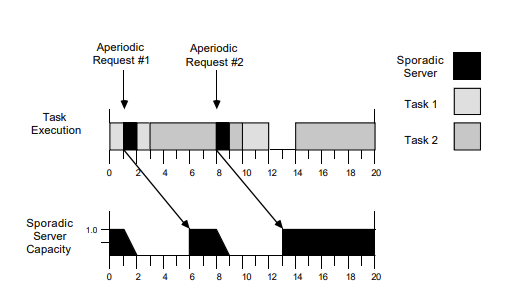
\includegraphics{high priority ss.png}
    \caption{SS with high priority example}
    \label{fig:high priority ss graph}
\end{figure}
\subsection{Schedulability}
Even though the sporadic server algorithm relies on the RM algorithm, it violates one of the basic assumptions laid out by Liu and Layland in their analysis of RM\cite{schedulingformula} which states "
\bibliographystyle{unsrt} 
\bibliography{refs}

\end{document}
